\documentclass[11pt]{article}
\usepackage[T1]{fontenc}
\usepackage[margin=1.1in]{geometry}
\usepackage{amsmath,amssymb,amsthm}
\usepackage{booktabs}
\usepackage{longtable}
\usepackage[ruled,vlined,linesnumbered]{algorithm2e}
%% upright comments: the default is italic, and Computer Modern has no
%% italic small caps, so \textsc inside a comment falls back silently.
\SetCommentSty{textnormal}
%% Algorithm identifiers. `\textnormal` first, because Computer Modern has no
%% italic small caps and an identifier inside an italic context falls back silently.
\newcommand{\proc}[1]{\textnormal{\scshape #1}}
\usepackage{array}
\usepackage{graphicx}
\usepackage{microtype}
\usepackage[colorlinks=true,linkcolor=blue,citecolor=blue,urlcolor=blue]{hyperref}

\newtheorem{proposition}{Proposition}
\newtheorem{lemma}{Lemma}
\theoremstyle{definition}
\newtheorem{definition}{Definition}
\theoremstyle{remark}
\newtheorem{remark}{Remark}

\newcommand{\code}[1]{\texttt{#1}}
\newcommand{\R}{\mathbb{R}}
\newcommand{\Om}{\Omega}
\newcommand{\lam}{\lambda}
\newcommand{\sig}{\sigma}
\newcommand{\pr}{\mathrm{prec}}
\newcommand{\abs}[1]{\left\lvert #1 \right\rvert}
\newcommand{\norm}[1]{\left\lVert #1 \right\rVert}
\DeclareMathOperator*{\argmin}{arg\,min}

%% ragged left-aligned p-column: justification in narrow columns stretches badly
\newcolumntype{P}[1]{>{\raggedright\arraybackslash}p{#1}}

\graphicspath{{figures/}}

\title{Bracketing eigenvalues from a tension curve\\
\large The mathematics of \texttt{chladni}'s v1 bracket search}
\author{chladni development notes}
\date{}

\begin{document}
\maketitle

\begin{abstract}
\noindent
The method of particular solutions turns the Dirichlet eigenvalue problem on a planar domain
into the problem of finding the local minima of a scalar \emph{tension} curve
$\sig_1(\lam)$, the smallest generalized singular value of a matrix pencil. This note
develops the algorithm \code{chladni} uses for the first half of that search: given a window
$[a,b]$ and a requested relative precision $\pr$, produce a set of intervals each believed
to contain one eigenvalue, and then drive each down to machine accuracy. Four ideas carry the
design. (i) Near an eigenvalue $\sig_1$ is a cone with a rounded bottom, whose two parameters
--- a floor $\varepsilon$ belonging to the \emph{basis} and a wall slope $c$ belonging to the
\emph{domain} --- are independent, and whose ratio $\varepsilon/c$ is the resolution limit.
(ii) The wall slope scales as $c(\lam)=C/\sqrt{\lam}$, which makes $k=\sqrt{\lam}$ the
\emph{unique} power of $\lam$ in which one Lipschitz bound serves a whole window; this change
of variable is worth more than every algorithmic change in the design combined. (iii) A
Lipschitz bound converts samples into intervals \emph{certified to contain no eigenvalue}, and
the cost of certifying a cone's wall is a geometric ladder whose ratio depends only on the
safety factor --- which fixes the cost of the method and retires a family of attempts to make
it cheaper. (iv) One evaluation returns the whole singular-value vector, so $\sig_2$ is free,
and $\sig_2/c$ is a distance meter that is accurate exactly where the decision is hard. We
derive each, state honestly what is proved and what is only measured, and record what changed
when the algorithm was ported from the repository it was designed in.
\end{abstract}

\tableofcontents

\section{What the bracketing stage is asked for}
\label{sec:problem}

\subsection{From the pencil to a scalar curve}

Let $\Om\subset\R^2$ be a bounded planar domain and consider the Dirichlet eigenvalue problem
$-\Delta u = \lam u$ in $\Om$, $u=0$ on $\partial\Om$. The method of particular solutions
(MPS) builds, at each trial value $\lam$, a basis $\psi_1(\cdot;\lam),\dots,\psi_n(\cdot;\lam)$
of functions that solve the Helmholtz equation $\Delta\psi + \lam\psi = 0$ in $\Om$
\emph{exactly}. Every member of the span is then an exact solution of the PDE, and only the
boundary condition remains to be satisfied. Sampling the boundary at $m_B$ collocation points
and the interior at $m_I$ points gives two matrices,
\[
  (A_B)_{ij} = \psi_j(x^B_i), \qquad (A_I)_{ij} = \psi_j(x^I_i),
\]
and the question ``is $\lam$ an eigenvalue?'' becomes ``is there a coefficient vector making
the boundary trace small without making the function small everywhere?'' That is measured by
the \emph{tension}
\begin{equation}\label{eq:tension}
  \sig_1(\lam) \;=\; \min_{c\neq0}\ \frac{\norm{A_B(\lam)\,c}}{\norm{A_I(\lam)\,c}},
\end{equation}
the smallest generalized singular value of the pencil $\bigl(A_B(\lam),A_I(\lam)\bigr)$. The
interior block is what stops the minimizer from returning the zero function; it is a
normalization, not a quadrature, and its only job is to keep $\norm{A_I c}$ away from zero.

Three properties of $\sig_1$ shape everything below.

\begin{enumerate}
\item \textbf{It dips to a floor at each eigenvalue and is $O(1)$ elsewhere.} The elevated
region between dips is the \emph{plateau}, and its height is the natural scale against which
smallness is judged.
\item \textbf{One evaluation returns the whole ascending vector}
$\sig_1\le\sig_2\le\cdots$. An eigenvalue of multiplicity $m$ drives $m$ of them to the floor
together, and reading $\sig_2$ costs nothing extra. Section~\ref{sec:gate} spends this.
\item \textbf{Evaluations are expensive.} One costs a QR, an SVD and a generalized SVD ---
5--70\,ms depending on basis size. Cost is therefore counted in evaluations and in nothing
else, and every design decision below is ultimately a decision about how many to spend.
\end{enumerate}

\subsection{The output contract, and its two metrics}

\begin{definition}[The bracketing problem]
Given the tension function, a window $[a,b]$ and a requested relative precision $\pr$,
return a set of non-overlapping intervals, each of which the method \emph{believes} contains
an eigenvalue.
\end{definition}

Two properties of the returned set are hard requirements.

\begin{description}
\item[Coverage.] Every eigenvalue in $[a,b]$ lies in some returned interval. A lost eigenvalue
cannot be recovered downstream by any amount of refinement, so this is the metric that governs.
\item[Purity.] No returned interval contains eigenvalues spanning more than $\pr\cdot\lam$.
An interval holding two eigenvalues the user asked to have separated is a wrong answer, not an
imprecise one.
\end{description}

Everything else --- how many intervals, how many of them are empty, what it all cost --- is
reported and traded rather than required.

\begin{remark}[The stage must commit]
The returned intervals are the ones the method believes hold an eigenvalue, \emph{not} a
subdivision of $[a,b]$. The distinction is not pedantic: a method that partitions the window
achieves perfect coverage for free and without evaluating anything, while a method that
commits covers a small fraction of the window and has to earn it. Without this rule the two
are not comparable at all.
\end{remark}

Note what purity does \emph{not} constrain: the \emph{width} of an interval holding a single
eigenvalue. Such an interval spans zero eigenvalues however wide it is. This observation is
worth remembering; it is the whole of \S\ref{sec:emit}'s argument for stopping early.

\section{The local model, and what its two parameters mean}
\label{sec:cone}

Near a simple eigenvalue $\lam^*$, the tension is well described by
\begin{equation}\label{eq:cone}
  \sig_1(\lam)\;\approx\;\sqrt{\varepsilon^2 + c^2\,(\lam-\lam^*)^2},
\end{equation}
a cone of slope $c$ with a rounded bottom of depth $\varepsilon$. On the four domains where it
has been checked --- rectangle, disk, equilateral triangle, L-shape --- \eqref{eq:cone} fits
the far field to a median relative residual of 1--3\%, failing only where the floor comes close
to the plateau, that is, where the basis cannot represent the eigenfunction at all.

The two parameters are independent, and \emph{which is which} matters more than either value.

\begin{description}
\item[$\varepsilon$ is the floor.] It is $\sig_1$ at the eigenvalue: the residual of the best
eigenfunction the finite basis can represent. It is dimensionless, and it is a property of
\textbf{the basis}.
\item[$c$ is the wall slope.] It is $d\sig_1/d\lam$ away from the eigenvalue, it carries units,
and it is a property of \textbf{the domain}.
\end{description}

Figure~\ref{fig:cone} is the evidence. On the L-shape with a Fourier--Bessel basis at the
reentrant corner, taking 20, 40 and 60 terms moves the floor from $4.0\times10^{-5}$ to
$1.1\times10^{-12}$ --- seven orders --- while the wall slope moves from $1.6022$ to $1.5951$,
four parts in a thousand. Enriching the basis deepens the well; it does not change its walls.

\begin{figure}[t]
  \centering
  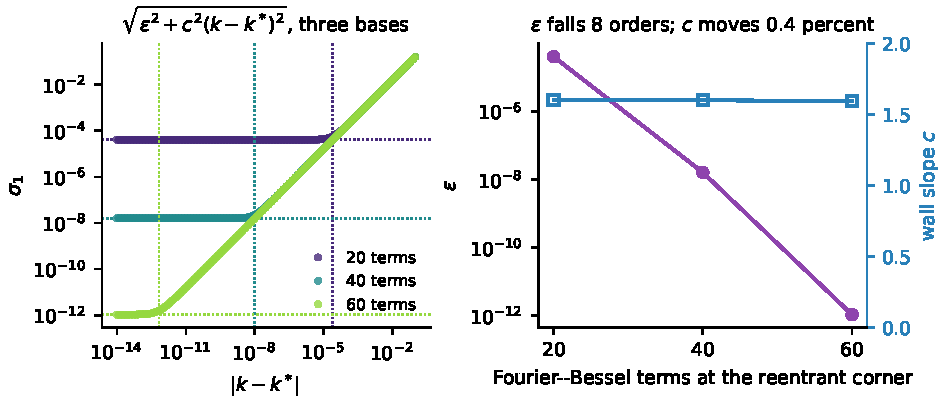
\includegraphics[width=\textwidth]{cone.pdf}
  \caption{The cone model on the L-shape, at the first eigenvalue, with a Fourier--Bessel basis
  at the reentrant corner. \emph{Left:} measured $\sig_1$ (points) against
  \eqref{eq:cone} (lines) for three basis sizes; dotted lines mark $\varepsilon$ and
  $\varepsilon/c$. The three curves share a wall and differ only in where they bottom out.
  \emph{Right:} the same three fits. Only $\varepsilon$ responds to the basis.}
  \label{fig:cone}
\end{figure}

\subsection{The resolution limit}

Setting $\lam-\lam^*=\varepsilon/c$ in \eqref{eq:cone} gives $\sig_1=\sqrt{2}\,\varepsilon$:
the ratio
\begin{equation}\label{eq:reslimit}
  \frac{\varepsilon}{c}
\end{equation}
is the scale at which the cone stops looking like a wall and starts looking like its own
rounded bottom. Two eigenvalues closer together than $\varepsilon/c$ have overlapping bottoms
and cannot be separated by \emph{any} method reading this curve, however many evaluations it
spends. Since $c$ is fixed by the geometry, $\varepsilon$ alone sets the limit --- which is the
concrete form of the statement that \emph{the search is bounded by the basis}. It is the
basis planner's job to make $\varepsilon$ small enough; it is the search's job to find
everything that is separated by more than about $20\,\varepsilon/c$, which is the quantitative
form of the contract between the two layers.

\begin{remark}[No absolute threshold on $\sig$ can serve as a test]
\label{rem:nothreshold}
The floor is not a single number even within one scan, and the reason is worth stating
precisely because a loose version of it is easy to repeat. At a corner of interior angle
$\omega$ the local expansion of an eigenfunction runs in
\[
  r^{\,l\pi/\omega}\,\sin\!\bigl(l\pi\theta/\omega\bigr), \qquad l = 1,2,\dots,
\]
whose exponents are fractional unless $\omega/\pi$ divides $l$. Every Dirichlet eigenfunction
\emph{vanishes} at the corner --- that is the boundary condition, and it distinguishes
nothing. What distinguishes one mode from another is whether the \emph{coefficients of the
fractional-exponent terms} vanish. A mode with no singular part is analytic there and a finite
basis represents it almost exactly; its neighbours carry the singularity and are represented
far less well. On the L-shape, $\omega=3\pi/2$ gives exponents $r^{2l/3}$, smooth only when
$3\mid l$; the mode at $\lam=2\pi^2$ is the unit square's fundamental
$\sin(\pi x)\sin(\pi y)$ tiled across the three cells, which vanishes on the whole integer
grid and is entire.

Every threshold in the algorithm is therefore stated as a fraction of the \emph{measured
plateau}, never as an absolute tension.

The measurement behind this rule has itself been corrected, and the correction is instructive.
An early measurement recorded a five-order floor spread on the L-shape --- $3.1\times10^{-13}$
at one level against $5.5\times10^{-8}$ at a neighbour --- and explained it structurally. With
a recipe-grade basis (80 pure Fourier--Bessel terms at the reentrant corner) the same levels
read within a factor of $4.2$ of one another, and the level previously at $5.5\times10^{-8}$
reads $5.3\times10^{-15}$. So the five orders were an artifact of an inadequate basis. The
\emph{design rule} survives either way, because a factor of four still defeats any fixed
constant and a domain whose basis cannot be made adequate will still show the large spread;
what does not survive is the claim that the L-shape is intrinsically such a domain.
\end{remark}

\section{Why the wavenumber, and why uniquely}
\label{sec:whyk}

This section contains the shortest derivation in the document and the one that decides the
most.

The cover phase of \S\ref{sec:cover} rests on a single Lipschitz bound $L$ used across a whole
window. Such a bound is conservative by the ratio of the largest local slope in the window to
the smallest, and it is paid \emph{everywhere}. Reducing that ratio is therefore the largest
available saving, and it is available before any algorithm has been chosen.

Measurement supplies the scaling: on the family where it was first taken,
\begin{equation}\label{eq:cscaling}
  c(\lam) \;=\; \frac{C}{\sqrt{\lam}}, \qquad C = 0.27 \pm 8\%,
\end{equation}
so $c$ varies by a factor of $4.81$ across $\lam\in[10,400]$. Now search not in $\lam$ but in
$u=\lam^p$ for some power $p$. By the chain rule,
\begin{equation}\label{eq:pderivation}
  \frac{d\sig}{du}
  \;=\; c(\lam)\,\frac{d\lam}{du}
  \;=\; \frac{C}{\sqrt{\lam}}\cdot\frac{\lam^{1-p}}{p}
  \;=\; \frac{C}{p}\,\lam^{1/2-p},
\end{equation}
which is constant in $\lam$ for $p=1/2$ and for no other power. This is not a fit; it is the
exponent that cancels.

\begin{proposition}
Under the scaling \eqref{eq:cscaling}, $u=\lam^{p}$ makes the wall slope independent of the
level if and only if $p=1/2$; that is, if and only if $u$ is the Helmholtz wavenumber
$k=\sqrt{\lam}$.
\end{proposition}

That $k$ is also the physical variable --- the wavenumber at which the basis functions are
built --- is the reason this is expected to transfer to other domains, rather than being a
property of the family it was measured on.

Figure~\ref{fig:whyk} confirms it on a different rectangle, in a different implementation, from
the one where \eqref{eq:cscaling} was measured. Over 17 isolated levels in $\lam\in[10,520]$,
the spread of $d\sig/du$ (standard deviation over mean) is 48\% in $\lam$, 22\% in
$\lam^{3/4}$, 17\% in $\lam^{1/4}$, 30\% in $\log\lam$, and \textbf{5.9\% in $k$}. The
originating measurement reported 57\%, 27\%, 17\%, 32\% and 5\%. Two independent
implementations, two different rectangles, the same answer.

\begin{figure}[t]
  \centering
  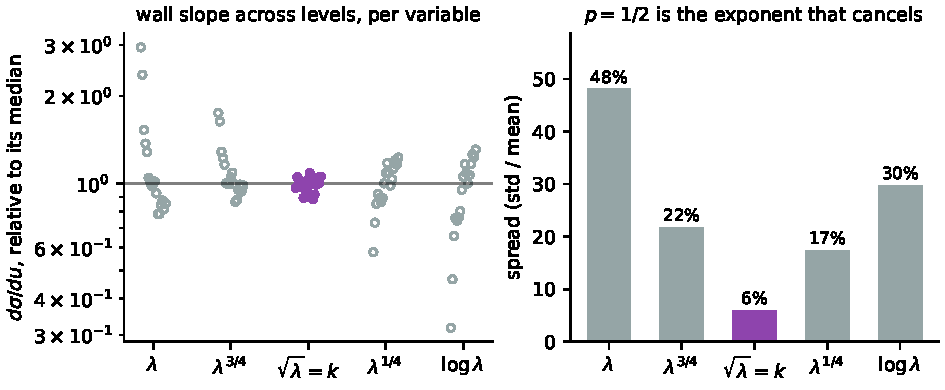
\includegraphics[width=\textwidth]{whyk.pdf}
  \caption{The wall slope across 17 isolated levels of a $1\times\varphi^{-1}$ rectangle,
  under five changes of variable. \emph{Left:} each level's slope relative to the median for
  that variable. \emph{Right:} the spread. The exponent that cancels is the one the data pick
  out.}
  \label{fig:whyk}
\end{figure}

\begin{remark}[How much this is worth]
In the design's own version history this change of variable accounts for a factor of $1.8$ out
of a total $2.6$ improvement --- more than every algorithmic change in the method combined. It
is worth stating plainly, because it is easy to read as a numerical detail and it is not one.
\end{remark}

\subsection{Two consequences of working in a transformed variable}

\paragraph{The precision factor.} Purity is judged on $d\lam$ against $\pr\cdot\lam$, but the
search contracts brackets in $u$. A bracket $[u_1,u_2]$ maps to $d\lam=(d\lam/du)\,du$, so for
$u=\lam^p$ the relative precision that must be met in $u$ is
\begin{equation}\label{eq:precu}
  \pr_u \;=\; p\cdot\pr,
\end{equation}
a \emph{half} for the wavenumber. Evaluated at the upper end of the bracket, so conservative.

\paragraph{The ulp slack.} The round trip $k\mapsto k^2$ is not exact. A bracket that correctly
fences $k^*$ can fail to fence $\lam^*=(k^*)^2$ after squaring, because an endpoint rounds the
wrong way; this was observed as a coverage loss of exactly one unit in the last place. Every
returned endpoint is therefore widened by about four ulps, and brackets that abut after
widening are merged.

\paragraph{And the refiner wants the other variable.} \S\ref{sec:refine} shows that the
quadratic fit the refinement performs is markedly better in $\lam$ than in $k$. The two stages
want two variables and they get them: \textbf{cover in $k$, refine in $\lam$}. This is not a
compromise between two measurements but the conclusion of both, and it is worth noticing that
the reasons are genuinely different --- the scan cares about the \emph{slope}, which is flat in
$k$, and the refiner cares about the \emph{curvature}, which is better behaved in $\lam$.

\section{Seeding the scan, and estimating the slope}
\label{sec:seed}

\subsection{Weyl sizes the grid and says nothing else}

Weyl's law with the perimeter correction,
\begin{equation}\label{eq:weyl}
  N(\lam) \;\sim\; \frac{\abs{\Om}\,\lam}{4\pi} \;-\; \frac{\abs{\partial\Om}\sqrt{\lam}}{4\pi},
\end{equation}
predicts the number of eigenvalues in a window to 1--11\% on the families tested. It is used
for exactly one thing: to set the starting sample density, at 1.5 samples per expected gap. It
says nothing whatever about \emph{where} anything is, and must never be used as though it did.

The starting density barely matters, because the doubling below adapts: 0.5, 1.0 and 1.5
samples per gap all cost the same. The larger is chosen for margin.

\subsection{Nested doubling, and why $n\to 2n$ is wrong}

The seed then doubles, inserting midpoints so that $n\to 2n-1$ and each grid \emph{contains}
the previous one exactly, until the largest observed secant slope stops growing by more than
10\%.

Exact nesting is not tidiness. Under $n\to 2n$ the new points land at irrational offsets from
the old ones, and some of them land within an ulp of an old point. A secant computed across
such a pair measures rounding, not slope: one such estimate reached $7.3\times10^{10}$ against
a true slope of $0.6$. Since the slope model is monotone non-decreasing (\S\ref{sec:slope}), a
model that once believes that can never recover. For the same reason, pairs closer than
$10^{-9}$ of the sampled span are excluded from the secant estimate altogether. Midpoint
insertion has a second benefit: the old points are reused bit-identically, so a doubling costs
only the genuinely new samples.

\subsection{The bootstrap hazard runs opposite to intuition}
\label{sec:bootstrap}

It is natural to worry that an \emph{over}estimated Lipschitz constant will make the search
expensive. The dangerous error is the other one. As \S\ref{sec:cover} will show, a sample of
value $v$ excludes a neighbourhood of radius $v/L$; an \emph{under}estimated $L$ makes those
radii too \textbf{large}, so a search that has not yet seen the true slope excludes everything
and terminates having found nothing --- silently, with no error at all. Measured, the largest
observed secant as a function of seed density, against a true slope of $0.0656$:
\begin{center}
\begin{tabular}{lrrrrrr}
\toprule
$n$ & 8 & 16 & 32 & 64 & 128 & 256\\
largest secant & 0.0046 & 0.0128 & 0.0386 & 0.0599 & 0.0647 & 0.0652 \\
as a fraction of the truth & 7\% & 20\% & 59\% & 91\% & 99\% & 99\% \\
\bottomrule
\end{tabular}
\end{center}
At $n=8$ the exclusion radii would be fourteen times too large.

Two things defuse this. First, the doubling itself: the estimate is not used until it has
stopped growing. Second, and more important, \emph{exclusions are recomputed from the current
$L$ on every pass}, so a subsequent growth in $L$ revives whatever that growth un-excludes. An
underestimate therefore costs extra work rather than causing a silent miss.

\begin{remark}[The bootstrap is the falsification test]
An estimate that never settles is not a nuisance to be worked around: it is the evidence that
nothing bounds the local slope on this curve, at any scale sampled. That is a legitimate ground
for the method to decline (\S\ref{sec:decline}), and it is the only such evidence available.
\end{remark}

\subsection{The slope model, and what it is honestly worth}
\label{sec:slope}

The model is
\begin{equation}\label{eq:L}
  L \;=\; s\cdot\max_{i}\ \abs{\frac{v_{i+1}-v_i}{x_{i+1}-x_i}}, \qquad s = 1.5,
\end{equation}
monotone non-decreasing over the run. The honesty clause must be stated before anything is
built on it.

\begin{proposition}[There is no certificate here]
\label{prop:nolipschitz}
No finite sample set bounds a Lipschitz constant from above. The largest observed secant is a
\emph{lower} bound on $\sup\abs{f'}$, and multiplying it by a safety factor produces a number
with no formal status.
\end{proposition}

This is not a defect that better engineering removes; it is a property of the information
available. The consequence is that every completeness claim the method makes is
\emph{conditional on $L$}, and must be reported as such (\S\ref{sec:claim}).

Two measurements set $s=1.5$, and they pull in opposite directions.

\begin{itemize}
\item \textbf{The bound is nearly tight, so it cannot be shaved.} On the window where it was
measured the largest observed secant reaches the true nearest eigenvalue exactly. Using the
99th-percentile slope instead of the maximum --- a 1.4\% reduction --- wrongly excluded 13 of
600 samples. Coverage is lost by very small underestimates.
\item \textbf{Margin is cheap in the seed.} Raising $s$ from 1.2 to 2.0 cost 40\% more
evaluations for identical coverage.
\end{itemize}

Finally, distinguish a \emph{surprise} growth --- $L$ rising after exclusions have already
relied on it --- from mere convergence of the estimate. A creep from $0.0647$ to $0.0656$ is
the estimate settling. Only surprises are counted, and a run with many of them deserves a rerun
at a larger $s$; it is not, by itself, wrong.

\subsection{An aside: could the scan have found it at all?}

Sizing the scan is a \emph{precondition}, not a diagnostic, and \code{chladni} ships a
closed-form check for it. Model the dip as a clipped V, $\sig\approx\min(\sig_{\text{base}},
C_k\abs{k-k_j})$, where $\sig_{\text{base}}$ is the plateau. Its visible width is
$w_k = 2q\,\sig_{\text{base}}/C_k$ for a visibility fraction $q$, and demanding that a scan of
stride $\Delta k$ resolve it, $w_k\ge\Delta k$, gives
\begin{equation}\label{eq:findability}
  \sig_{\text{base}} \;\ge\; \frac{\kappa}{2q}\cdot\frac{\abs{\Om}}{\abs{\partial\Om}}\cdot\Delta k,
  \qquad \kappa \;=\; \frac{C_k}{\abs{\Om}/\abs{\partial\Om}} .
\end{equation}
The $\abs{\Om}/\abs{\partial\Om}$ scaling is confirmed exactly: the same $3\!:\!1$ rectangle at
scales $0.5$, $1$, $2$ gives $C_k/(A/P) = 2.4600,\ 2.4600,\ 2.4598$, while $C_k/A$ varies by a
factor of four over the same three. The dimensionless $\kappa$ transferred between two
independent implementations within one standard deviation, $2.591\pm0.226$ against
$2.384\pm0.231$.

\section{Cover by exclusion}
\label{sec:cover}

\subsection{The Piyavskii bound}

Suppose $f$ is $L$-Lipschitz and we know $f(x_i)=v_i$ and $f(x_j)=v_j$ at two adjacent samples,
$x_i<x_j$, $h=x_j-x_i$. Then for every $x\in[x_i,x_j]$,
\begin{equation}\label{eq:pbound}
  f(x) \;\ge\; \max\bigl\{\,v_i - L(x-x_i),\ \ v_j - L(x_j-x)\,\bigr\},
\end{equation}
the pointwise maximum of two cones of slope $L$ dropping from the two samples. The right-hand
side is minimized where the two branches cross, giving

\begin{lemma}[The envelope and its minimizer]
\label{lem:envelope}
The bound \eqref{eq:pbound} attains its minimum
\begin{equation}\label{eq:env}
  \hat{s} \;=\; \frac{v_i+v_j-Lh}{2}
  \qquad\text{at}\qquad
  \hat{x} \;=\; \frac{x_i+x_j}{2} + \frac{v_i-v_j}{2L}.
\end{equation}
\end{lemma}

\begin{proof}
The two branches are affine with slopes $-L$ and $+L$; their maximum is minimized at their
crossing, $v_i-L(x-x_i)=v_j-L(x_j-x)$, which rearranges to $\hat x$ above and gives the value
$\hat s$ by substitution.
\end{proof}

Two consequences, and the method is built from them.

\begin{description}
\item[The exclusion certificate.] If $\hat s\ge0$ then $f>0$ throughout $(x_i,x_j)$, so no
eigenvalue lies between the two samples. The cell is \emph{certified empty} --- conditional on
$L$, per Proposition~\ref{prop:nolipschitz}.
\item[Where to look next.] $\hat x$ is the point attaining the bound: the most informative
place in the cell, and where the search samples.
\end{description}

Cells not excluded are \emph{live}, and contiguous live cells are merged into \emph{regions}.
Merging matters: the two cells either side of an eigenvalue are both live, and reported
separately they would look like two candidates where there is one.

Figure~\ref{fig:exclusion} shows the construction on a real tension curve.

\begin{figure}[t]
  \centering
  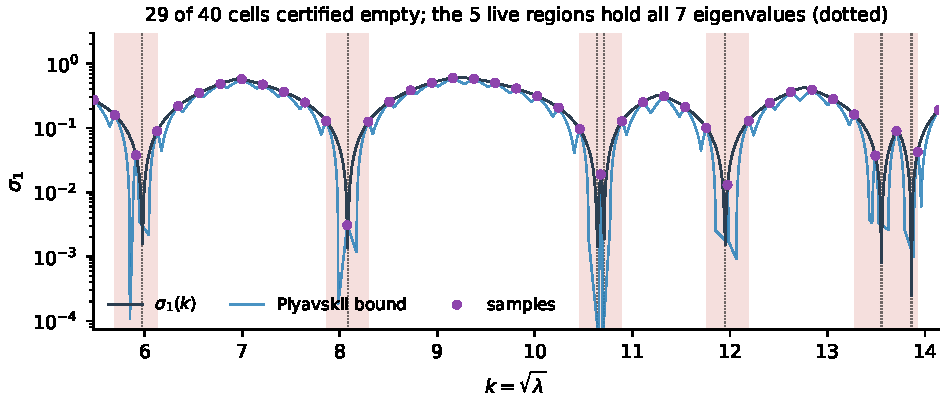
\includegraphics[width=\textwidth]{exclusion.pdf}
  \caption{Cover by exclusion on a $1\times\varphi^{-1}$ rectangle,
  $\lam\in[30,200]$, from 41 uniform samples with $L=1.5\times$ the largest observed secant.
  The sawtooth is the Piyavskii bound \eqref{eq:pbound}, drawn only where it is positive. 29 of
  40 cells are certified empty; the five surviving live regions (shaded) contain all seven
  eigenvalues (dotted). Two of them hold a pair, which is what \S\ref{sec:gate} exists to
  detect.}
  \label{fig:exclusion}
\end{figure}

\begin{remark}[The zero threshold, and why it does not need to be raised]
\label{rem:zerothreshold}
The test $\hat s\ge 0$ presumes $\sig_1$ reaches zero at an eigenvalue, and it does not: it
bottoms at $\varepsilon>0$. So as the spacing shrinks the bound rises toward a positive value
and a sufficiently finely sampled well could, in principle, exclude \emph{itself}. This is a
reasonable objection and the answer is structural rather than a tuned constant: the cover loop
stops on purity-by-width long before that regime is reached, so the zero threshold never bites.
Replacing it with a positive threshold was tried and broke every case --- 0 of 66.
\end{remark}

\subsection{The cost law}
\label{sec:ladder}

What does it cost to certify a cone's wall as empty? Take two samples on the same wall at
distances $u_a>u_b$ from the eigenvalue, so their values are $c\,u_a$ and $c\,u_b$, and take
$L=s\,c$. By \eqref{eq:env} the cell between them is excluded when
\[
  \frac{c(u_a+u_b)}{2} - \frac{s\,c\,(u_a-u_b)}{2} \;\ge\; 0
  \quad\Longleftrightarrow\quad
  (1-s)\,u_a + (1+s)\,u_b \;\ge\; 0,
\]
that is, when
\begin{equation}\label{eq:ladder}
  \frac{u_b}{u_a} \;\ge\; \frac{s-1}{s+1}.
\end{equation}

\begin{proposition}[The ladder]
\label{prop:ladder}
The condition \eqref{eq:ladder} is independent of $c$. A cone's wall is therefore covered by a
\emph{geometric ladder} of samples with ratio at most
\[
  r(s) \;=\; \frac{s+1}{s-1},
\]
and covering a range of scales $R$ costs $\log R/\log r(s)$ samples per side.
\end{proposition}

Two things about this deserve emphasis. It is independent of the wall slope, so it holds
uniformly over the window and over domains. And it is exact: Figure~\ref{fig:ladder} recovers
$r(s)$ to five figures by bisecting on the ratio against the exclusion code itself.

\begin{figure}[t]
  \centering
  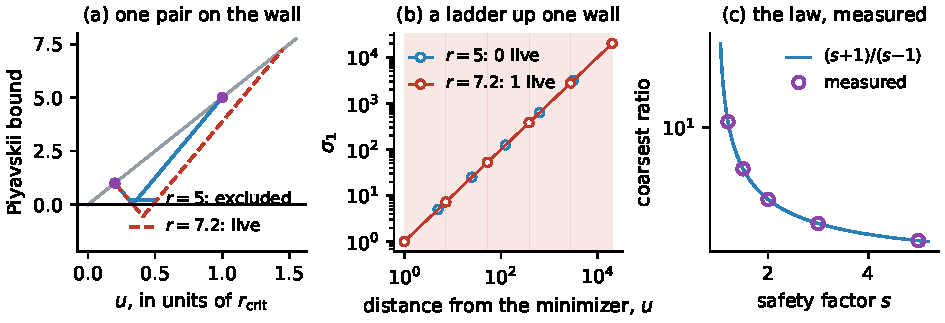
\includegraphics[width=\textwidth]{ladder.pdf}
  \caption{\emph{(a)} One pair on a wall. At the critical ratio the Piyavskii bound just
  touches zero; past it the bound dips below and the cell stays live. \emph{(b)} A ladder up
  one wall: at $r=5$ every cell is excluded, at $r=7.2$ none is. \emph{(c)} The ratio measured
  by bisection against \code{live\_regions}, against $(s+1)/(s-1)$.}
  \label{fig:ladder}
\end{figure}

\begin{remark}[A better prediction cannot help the cover phase]
\label{rem:noprediction}
Proposition~\ref{prop:ladder} retires a family of ideas. Placing a sample \emph{exactly on} an
eigenvalue leaves the live region completely unchanged, and so does placing two that straddle
it to within $10^{-9}$: what is live is the \emph{wall}, and the wall yields to the ladder or
to nothing. Six separate attempts to make cover cheaper by sampling more cleverly all failed
for this one reason, and a seventh would too. Cleverness about \emph{where the eigenvalue is}
belongs in the locator (\S\ref{sec:locate}), not here.
\end{remark}

\begin{remark}[A larger safety factor is a finer ladder]
Raising $s$ does not merely buy margin; it costs $1/\log r(s)$ per side, so the cover phase's
cost grows as $s$ rises. That is why the tension in \S\ref{sec:slope} between ``the bound is
nearly tight'' and ``margin is cheap'' is a real trade and not a free choice.
\end{remark}

\subsection{Why adapt at all}

A uniform grid must resolve the tightest pair it might meet. A pair at separation $d$ is
resolved once the sampling near it is finer than about $d/3$, so a uniform grid over $[a,b]$
needs $n\sim 3(b-a)/d$ samples \emph{everywhere}, while exclusion refines only where $\sig_1$
is small and costs $O(\log(1/d))$. Measured on an interval of width 2:
\begin{center}
\begin{tabular}{lrrr}
\toprule
$d$ & uniform grid & exclusion & ratio\\
\midrule
$3\times10^{-3}$ & $2048$ & 47 & $43\times$\\
$10^{-4}$ & ${\sim}6\times10^{4}$ & 57 & $1053\times$\\
$10^{-6}$ & ${\sim}6\times10^{6}$ & 71 & $8.5\times10^{4}$\\
$10^{-10}$ & ${\sim}6\times10^{10}$ & 97 & $6\times10^{8}$\\
\bottomrule
\end{tabular}
\end{center}
The comparison matters because $d$ is \emph{not known in advance}. A black-box solver cannot
tune its grid to the tightest pair it will meet, so the uniform-grid column is a cost it would
have to pay everywhere and forever, against a pair it may or may not have.

\section{The isolation gate: what $\sig_2$ buys}
\label{sec:gate}

\subsection{Why a gate is needed}

Once a region is believed to hold one eigenvalue, a fast locator can drive it down cheaply.
But a locator that converges to a single minimizer will happily converge to \emph{one member of
a close pair} and leave the other outside the bracket it returns. This is not hypothetical: it
is exactly how a grid-then-bisect baseline falls from coverage $1.0$ to $0.577$. The fast path
must therefore be gated, and the gate must be right.

\subsection{The signal, and why it is conservative by construction}

One evaluation returns the whole ascending vector, so $\sig_2$ is free. Near an eigenvalue,
$\sig_2$ is the second branch of the pencil --- which, at a simple level, is the \emph{next}
eigenvalue's cone --- so
\begin{equation}\label{eq:meter}
  \frac{\sig_2(x)}{c} \;\approx\; \text{distance from $x$ to the next eigenvalue}.
\end{equation}
A region is certified to hold one eigenvalue when
\begin{equation}\label{eq:gatetest}
  \text{neighbour} \;>\; \gamma\cdot(\text{region width}), \qquad \gamma=1.5.
\end{equation}

The estimator's error structure is what makes this safe, and it is worth stating carefully.
Measured against the true gap, \eqref{eq:meter} reads at ratio $0.97$--$1.03$ when the
neighbour is close, and $0.78$--$1.30$ when it is far (Figure~\ref{fig:gate}). It is accurate
\emph{precisely where the decision is hard} --- when a neighbour is close enough to be a purity
risk --- and where it is inaccurate it generally \emph{under}-reads the gap. A gate phrased as
``is the neighbour further away than this region is wide?'' therefore errs toward refusing to
certify. It is conservative by construction, not by tuning.

\begin{figure}[t]
  \centering
  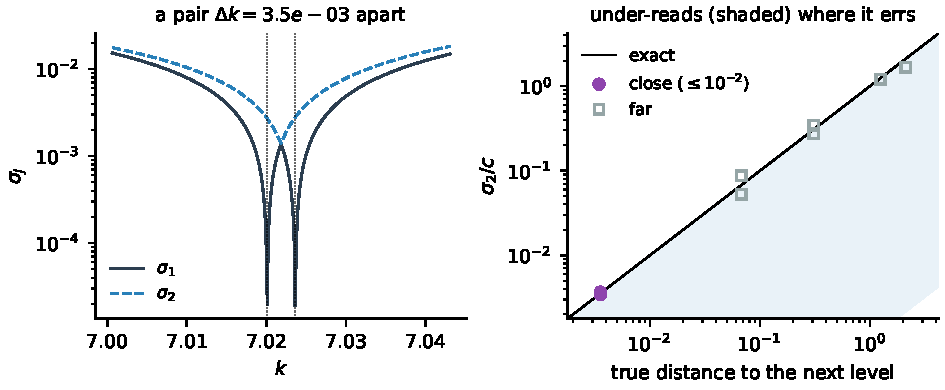
\includegraphics[width=\textwidth]{gate.pdf}
  \caption{\emph{Left:} $\sig_1$ and $\sig_2$ across a resolved pair on a
  $(1+\delta)\times1$ rectangle. $\sig_2$ has a single minimum, at the crossing point.
  \emph{Right:} the reading $\sig_2/c$ against the true distance to the next level, over nine
  levels of two pencils, computed by the searcher's own \code{isolation} routine. The shaded
  half-plane is where the meter under-reads.}
  \label{fig:gate}
\end{figure}

\subsection{Estimating $c$ without cancellation}

The gate needs $c$, and it reads it off the descent triple. If sampled points $\text{lo} <
\text{mid} < \text{hi}$ straddle the minimizer then, on a cone,
$v_{\text{lo}} = c(\lam^*-\text{lo})$ and $v_{\text{hi}} = c(\text{hi}-\lam^*)$, so adding,
\begin{equation}\label{eq:clocal}
  c \;=\; \frac{v_{\text{lo}} + v_{\text{hi}}}{\text{hi}-\text{lo}} .
\end{equation}
No subtraction of nearly equal quantities appears anywhere, and the estimate does not depend on
where $\lam^*$ is within the triple.

\subsection{Four rules, each of which cost a measured failure}

\begin{enumerate}
\item \textbf{Judge the region, not the triple inside it.} The region is what gets handed to
the locator and can be several times wider than the certificate triple. A pair
$8.4\times10^{-4}$ apart was certified inside a region $1.24\times10^{-3}$ wide, and then
collapsed onto one member.

\item \textbf{$c$ must be an independent \emph{upper} bound}, taken as
$\max(c_{\text{local}}, L)$. Where a region holds \emph{two} eigenvalues its flanks span both
cones, so $\text{hi}-\text{lo}$ in \eqref{eq:clocal} is too wide, $c$ comes out too small, the
neighbour appears further away than it is, and the gate certifies precisely what it must not.
Trusting the local estimate alone cost 3 of 26 eigenvalues.

This is worth dwelling on, because the instinct is the reverse. Replacing the crude global $L$
with a \emph{learned} wall slope --- an obviously better estimate --- loses 12 of 19 cases. A
smaller slope makes the estimated neighbour distance larger, which pushes the gate toward
certifying. The global bound's apparent excess conservatism \emph{is} the safety margin.

\item \textbf{Silence is not permission.} If no descent certificate exists in the region there
is no decision to be had, and the region stays on the slow path. ``I cannot tell'' must not be
recorded as ``yes''.

\item \textbf{Do not read the level's multiplicity off the $\sig$ vector here.} Counting
branches at the floor and reading the first one that is not is correct \emph{in principle} ---
at a multiplicity-2 level, $\sig_2$ is that level's own second branch, and the next distinct
level is reported by $\sig_3$ --- and it saves 40\% on exactly degenerate cases. It is also
ambiguous at range by construction: approaching an unresolved pair of separation $d$ from
distance $u$,
\begin{equation}\label{eq:ambiguous}
  \frac{\sig_2}{\sig_1} \;=\; 1 + \frac{d}{u},
\end{equation}
which is $1.0006$ at the start of a cover pass. No threshold separates that from a genuine
multiplicity-2 level. Swept over two windows, the failure count is \textbf{not monotone} in the
threshold --- $0,1,0,1,2$ failures at $1.0,1.05,1.2,1.5,2.0$ --- and a parameter whose safety
alternates as it is tightened has no safe setting, only settings that pass the cases tried.
\end{enumerate}

\begin{remark}[The reading is not wrong; its placement was]
Read \emph{after} location, against a deliberately wide bracket, the same quantity is
unambiguous: 14 levels, 14 correct multiplicity readings, at zero additional evaluations,
because every point needed is already in the cache. Within a multiplet the ratio
$\sig_{j+1}/\sig_j$ runs $1.0$--$1.7$ and across the gap $10^{11}$--$10^{15}$, so a threshold of
$10$ is not a delicate parameter at all. What \eqref{eq:ambiguous} forbids is reading it
\emph{at range}, which is the only place the bracketer could.
\end{remark}

\section{Locate: predict, then straddle}
\label{sec:locate}

\subsection{The prediction is exact, and it is not enough}

Under the cone model \eqref{eq:cone},
\begin{equation}\label{eq:quad}
  \sig_1^2 \;=\; \varepsilon^2 + c^2(\lam-\lam^*)^2
\end{equation}
is \emph{exactly} quadratic. Three points therefore determine the minimizer exactly rather than
approximately, and the residual error comes only from the two branches meeting at the bottom
having slightly different slopes. This is also far better conditioned than the obvious
alternative of extrapolating a wall to zero, which subtracts nearly equal values.

Squaring is not a numerical sin here; see Remark~\ref{rem:squaring}.

Now the insight that makes the locator work.

\begin{remark}[Prediction alone does not tighten a bracket]
\label{rem:straddle}
A bracket needs sampled points on \emph{both} sides of the minimizer, so its width is set by
whichever side of the prediction has no sample near it. The prediction error has a
\emph{systematic sign}, because the two branches have slightly different slopes. So every
scheme that samples \emph{at} the prediction converges from one side only, and the far flank
never moves.
\end{remark}

The fix is to place the sample a fixed fraction of the bracket to one side of the prediction,
on whichever side is not already fenced. Each round of two such samples shrinks the bracket to
about $2\times$ the straddle fraction. That fraction is bounded below by the prediction error
--- an offset smaller than the error lands on the wrong side and the triple stops being a
descent --- and above by the contraction it buys.

Figure~\ref{fig:straddle} measures both bounds. The parabola's vertex lands within
$1.2\times10^{-4}$ of the truth at the median and $3.1\times10^{-3}$ at the 90th percentile, as
fractions of the bracket; the cost rises steadily with the offset above that. The shipped value
$0.02$ sits about six times above the measured 90th percentile of the prediction error, and
costs 14 evaluations against 12 at $0.01$ on this pencil.

\begin{figure}[t]
  \centering
  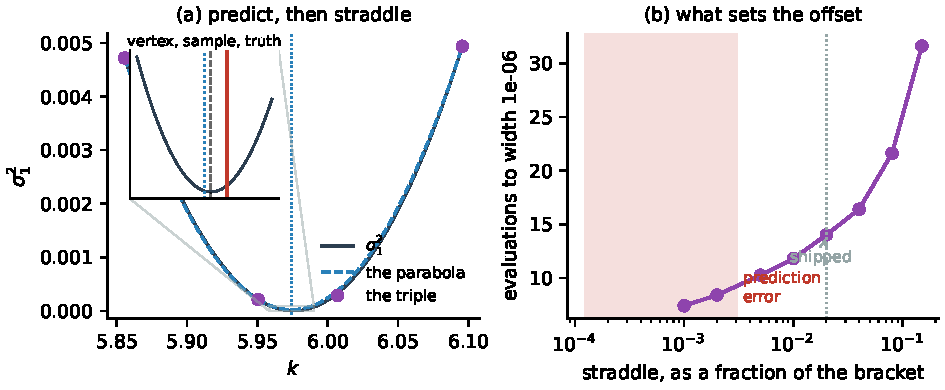
\includegraphics[width=\textwidth]{straddle.pdf}
  \caption{\emph{(a)} One locator step. $\sig_1^2$ and the parabola through the triple are
  indistinguishable at full scale; the inset zooms on the bottom, where the predicted vertex
  (dotted), the sample placed 2\% to its unfenced side (solid) and the true minimizer (dashed)
  separate. \emph{(b)} Evaluations to contract a bracket to width $10^{-6}$, averaged over five
  isolated levels, against the straddle fraction. The shaded band is the measured prediction
  error over the same runs, median to 90th percentile: below it the offset is inside the
  noise of the prediction.}
  \label{fig:straddle}
\end{figure}

\begin{remark}[Three designs that fail, each plausible]
Plain interpolation --- sampling at the prediction --- stalled with the bracket stuck.
Bisecting the lopsided side cured the stall but cost no less than exclusion. Mirroring the near
sample across the prediction oscillated without converging. Each is a natural thing to try, and
each is worth knowing has been tried.
\end{remark}

\subsection{What licenses emitting a bracket}
\label{sec:emit}

\begin{description}
\item[Every endpoint must be sampled, and carry a descent certificate.] For three sampled
points $p<q<r$ with $f(p)>f(q)<f(r)$, continuity alone gives a local minimum in $(p,r)$.
Nothing weaker may define an endpoint. In particular an \emph{extrapolated} root may not:
two-point secant roots fitted from opposite walls of a close pair were measured to
\textbf{cross} --- the left root landing to the right of the right root --- yielding an inverted
bracket, or a sliver containing nothing. Extrapolation may choose \emph{where to sample}; it
may not name an endpoint.
\end{description}

Two details of the certificate are easy to get wrong, and were.

\begin{itemize}
\item \textbf{Anchor on the region's lowest sample}, not on the deepest-looking triple. This is
what makes the bracket tighten monotonically: every new sample nearer the bottom becomes the
new centre, and its immediate neighbours are necessarily closer than the old ones. Selecting by
depth instead stalls, because depth tends to $1$ as the flanks approach the middle.
\item \textbf{Immediate neighbours only.} A descent read off non-adjacent samples would skip
whatever lies between them, and could straddle two cones with a barrier in between.
\end{itemize}

\paragraph{Depth, normalized by the further flank.} To decide whether a region holds a
minimizer at all, the middle's value is compared to its flanks. The normalization must be by
the \emph{larger} of the two flanking values. Using the nearer one systematically rejects real
eigenvalues: when a cone bottoms out near the middle of a sampling cell its two flanking
samples are almost equidistant, so their values are almost equal and the ratio approaches $1$
however deep the cone actually is. That cost 27\% of coverage --- 19 of 26 eigenvalues instead
of 26 --- \emph{at every grid density}, because refining the grid only moves the problem to a
different cell. Against the further flank, a mid-cell cone scores about $0.33$ while plateau
ripple still scores about $0.98$, which is the separation the ratio is for. The test is asked
\emph{once} per region, and never to choose among certificates: depth necessarily tends to $1$
as a bracket tightens, so a locator that filtered on it would stall partway down.

\subsection{Stop at isolation}

Recall from \S\ref{sec:problem} that purity does not constrain the width of a bracket holding
one eigenvalue. Refining past isolation therefore buys nothing the contract asks for, and the
refiner of \S\ref{sec:refine} reaches machine precision from a wide bracket in about seven
evaluations. So the bracket is handed on once the neighbour is four bracket-widths clear.

State plainly what this gives up. A bracket narrower than $\pr\cdot\lam$ cannot be impure
\emph{however wrong the gate was}; that unconditional guarantee is traded away, and purity then
rests on \S\ref{sec:gate}. This is the change in the design most in need of confirmation on
domains beyond the one it was measured on.

\begin{remark}[$\pr$ is a stopping rule, not a merge licence]
The search never reasons about whether merging two nearby eigenvalues into one bracket is
\emph{permitted}. The economics are entirely one-sided: merging saves the refinement of one
bracket, certifying that a merge is legal means resolving both eigenvalues anyway, and being
wrong is a hard purity failure. So the merges the search performs are only the ones it could
not resolve, and splitting beyond the licence is explicitly not an error.
\end{remark}

\section{The algorithm assembled}
\label{sec:assembled}

Every ingredient is now defined, and it is worth seeing them composed before the refinement
stage is added, because two structural facts are visible in the control flow and invisible in
the prose.

\paragraph{One loop, not two.} The obvious structure --- cover the window to find candidates,
then refine each candidate separately --- is wrong, and the baselines measure how wrong. Any
per-candidate refiner anchored on ``the lowest point I can see'' converges on one member of a
close pair and leaves the other outside the interval it returns; this is exactly how
grid-then-bisect falls from coverage $1.0$ to $0.577$. So cover and locate \emph{alternate},
and they operate on \emph{regions} rather than on candidate points. A region holding two
eigenvalues then splits of its own accord, the moment a sample placed between them is excluded.

\paragraph{The gate is asked three times.} It is consulted to decide whether a region may leave
the cover loop (Algorithm~\ref{alg:cover}, line~\ref{ln:gate1}), again after \emph{every}
locator step (Algorithm~\ref{alg:locate}, line~\ref{ln:gate2}), and once more on the way out
(line~\ref{ln:gate3}). Each catches a different failure, and all three are free: the gate is a
pure function of samples already paid for.

That last point is worth stating as a rule, because it explains the shape of the whole
algorithm.

\begin{remark}[Only one line spends anything]
In all three routines the sole operation that costs an evaluation is \proc{Evaluate}.
\proc{LiveRegions}, \proc{DescentCertificate}, \proc{Gate}, \proc{LocatorStep} and
\proc{LooksLikeADip} are pure functions of the sample arrays. This is why the design can
afford to re-ask expensive-sounding questions at every step, and why the cost accounting in
\S\ref{sec:claim} counts cache \emph{misses} and nothing else.
\end{remark}

\begin{algorithm}[H]
\caption{\proc{Bracket} --- the top level}
\label{alg:bracket}
\SetKwInOut{Input}{input}\SetKwInOut{Output}{output}
\Input{tension oracle $f(x)\mapsto(\sig_1,\sig_2,\dots)$; window $[a,b]$; precision $\pr$}
\Output{brackets in $\lam$, with diagnostics --- or a decline}
work in $k=\sqrt{\lam}$; \quad $\pr_u \leftarrow \pr/2$
  \tcp*{\eqref{eq:precu}}
$(X,V,\text{settled}) \leftarrow \proc{Seed}(f,a,b)$
  \tcp*{Weyl density, then nested doubling, \S\ref{sec:seed}}
\lIf{$\lnot\,\text{settled}$}{\Return $\proc{Decline}$(``nothing bounds the local slope'')}
$S \leftarrow \operatorname{median}(V)$
  \tcp*{the plateau, measured once; Rem.~\ref{rem:nothreshold}}
$L \leftarrow s\cdot\max_i \abs{(V_{i+1}-V_i)/(X_{i+1}-X_i)}$
  \tcp*{\eqref{eq:L}, $s=1.5$}
$\text{budget} \leftarrow 600 \cdot \max\bigl(N(b)-N(a),\,1\bigr)$
  \tcp*{per eigenvalue, never flat}
$\text{floorLimited}\leftarrow\proc{false}$\;
\For{$\text{round} \leftarrow 1$ \KwTo $5$}{
  $(X,V,L,\mathcal{R},\text{stalled}) \leftarrow \proc{Cover}(\dots)$
    \tcp*{Alg.~\ref{alg:cover}}
  $\text{floorLimited} \leftarrow \text{floorLimited} \lor \text{stalled}$\;
  $(X,V,\mathcal{R},\text{reopened}) \leftarrow \proc{Locate}(\dots)$
    \tcp*{Alg.~\ref{alg:locate}}
  \lIf{$\text{reopened}=0$}{\textbf{break}}
}
$\mathcal{K} \leftarrow \proc{Confirm}(X,V,\mathcal{R},L,S)$
  \tcp*{Alg.~\ref{alg:locate}}
\Return each $(a',b')\in\mathcal{K}$, widened by $4\,\mathrm{ulp}$ and mapped back by
  $u\mapsto u^2$, merging any that then abut
  \tcp*{\S\ref{sec:whyk}}
\end{algorithm}

\begin{algorithm}[H]
\caption{\proc{Cover} --- refine by exclusion until every region is settled}
\label{alg:cover}
\SetKwInOut{Output}{output}
\Output{samples, a possibly larger $L$, the live regions, and whether the floor bound}
\While{\textnormal{true}}{
  $\mathcal{R} \leftarrow \proc{LiveRegions}(X,V,L)$
    \tcp*{cells with $\hat s<0$, merged; \eqref{eq:env}}
  $\mathcal{T} \leftarrow \{\,R\in\mathcal{R} \;:\; \lnot\,\proc{PureByWidth}(R,\pr_u)
     \ \land\ \lnot\,\proc{Gate}(R,L)\text{ certifies single}\,\}$
    \label{ln:gate1}
    \tcp*{silence is not permission}
  \lIf{$\mathcal{T}=\varnothing$}{\Return $\mathcal{R}$, \proc{false}}
  \If{no reduction in $\sum_{\mathcal{T}}\abs{R}$ for 200 steps \textbf{or} budget spent}{
    \Return $\mathcal{R}$, \proc{true}
      \tcp*{floor-limited, \emph{not} a decline; \S\ref{sec:decline}}
  }
  $i \leftarrow \argmin\{\,\hat s_i \;:\; \text{cells } i \text{ of } \mathcal{T}\,\}$
    \tcp*{the deepest unexplained dip}
  $x \leftarrow \hat x_i$; \quad \proc{Evaluate} $f$ at $x$ and insert into $(X,V)$
    \tcp*{the Piyavskii point, \eqref{eq:env}}
  \lIf{$x$ was already a sample}{\Return $\mathcal{R}$, \proc{true}}
  \If{$s\cdot\max\text{secant} > L$}{
    $L \leftarrow s\cdot\max\text{secant}$; \quad $\text{growths} \mathrel{+}= 1$
      \tcp*{exclusions are recomputed next pass}
    \lIf{$\text{growths}>16$}{\Return $\proc{Decline}$(``the slope estimate keeps growing'')}
  }
}
\end{algorithm}

\begin{algorithm}[H]
\caption{\proc{Locate}, then \proc{Confirm}}
\label{alg:locate}
\SetKwProg{Fn}{procedure}{:}{}
\Fn{\proc{Locate}$(X,V,\mathcal{R},\pr_u,L)$}{
  \ForEach{region $(a_0,b_0)\in\mathcal{R}$}{
    \lIf{$\proc{PureByWidth}$ \textbf{or} $\lnot\,\proc{Gate}$ certifies single}{
      keep $(a_0,b_0)$; \textbf{continue}}
    $(a,b)\leftarrow(a_0,b_0)$\;
    \Repeat{at most 200 times, within budget}{
      $x \leftarrow \proc{LocatorStep}(X,V,a,b)$
        \tcp*{vertex of $\sig_1^2$, then straddle; \S\ref{sec:locate}}
      \lIf{$x$ is \proc{none} \textbf{or} already sampled}{\textbf{break}}
      \proc{Evaluate} $f$ at $x$; update $(a,b)$ to the new certificate\;
      $g \leftarrow \proc{Gate}\bigl((a,b),L\bigr)$
        \label{ln:gate2}
        \tcp*{free, and the answer changes}
      \lIf{$g.\text{neighbour} \le b_0-a_0$}{\textbf{break}
        \tcp*[f]{a pair after all}}
      \lIf{$g.\text{single} \ \land\ g.\text{neighbour} \ge 4\,(b-a)$}{\textbf{break}
        \tcp*[f]{isolated; hand it on}}
    }
    $g \leftarrow \proc{Gate}\bigl((a,b),L\bigr)$\;
    \eIf{$g$ is \proc{none} \textbf{or} $g.\text{neighbour} \le b_0-a_0$}{
      \label{ln:gate3}
      keep $(a_0,b_0)$; \quad $\text{reopened} \mathrel{+}= 1$
        \tcp*{too wide beats being wrong}
    }{
      keep $(a,b)$\;
    }
  }
}
\BlankLine
\Fn{\proc{Confirm}$(X,V,\mathcal{R},L,S)$}{
  \ForEach{region $(a,b)\in\mathcal{R}$}{
    \Repeat{3 times, or until a certificate exists}{
      \proc{Evaluate} $f$ at the Piyavskii point of the deepest cell in $(a,b)$
        \tcp*{not the widest gap}
    }
    keep $(a,b)$ \textbf{if} $\proc{DescentCertificate}$ exists,
      \textbf{or} $\min V \le \tfrac12\max V$ within it,
      \textbf{or} $\min V \le \tfrac12 S$
      \tcp*{the last disjunct: a region inside a well reads flat}
  }
}
\end{algorithm}

\subsection{Reading the algorithm}

Four lines carry most of the design, and each was arrived at by a measured failure.

\begin{itemize}
\item \textbf{The \proc{todo} filter} (Alg.~\ref{alg:cover}, line~\ref{ln:gate1}) has two
disjuncts because a region may leave the cover loop for two quite different reasons: it is
narrow enough that it \emph{cannot} be impure whatever it holds, or the gate has certified that
it holds one eigenvalue. A region the gate cannot judge satisfies neither and stays.

\item \textbf{The two non-decline exits} in Alg.~\ref{alg:cover} --- stalling, and asking for a
point that is already a sample --- return the regions in hand with a flag rather than an error.
They mean the objective's floor is binding, which is a fact about the pencil and not a failure
of the search.

\item \textbf{The reopen path} (Alg.~\ref{alg:locate}, line~\ref{ln:gate3}) discards the
locator's work and returns the \emph{original} region. It is what keeps the coverage guarantee
when the gate was wrong, and it is why the top level loops at all: the re-opened region goes
back through \proc{Cover}, where the locator's own samples now sit beside one member of the
pair and make exclusion cheap.

\item \textbf{The third disjunct in \proc{Confirm}} exists because a region lying entirely
\emph{inside} a well has every sample on the floor, so its internal ratio is $\approx1$ and it
reads as flat. Flatness at the floor is the opposite of flatness on the plateau, which is why
the test is a fraction of the measured $S$ (Remark~\ref{rem:nothreshold}).
\end{itemize}

Finally, note what is \emph{not} in the pseudocode: any reasoning about whether two nearby
eigenvalues may be merged. The search never decides that. It contracts until a region is pure
by width or certified single, and the merges it performs are only the ones it could not
resolve.

\section{Refinement}
\label{sec:refine}

The bracket is now handed to a refiner, which drives it to the requested accuracy.

\subsection{Iterated parabolic interpolation, not Brent}

Because \eqref{eq:quad} is exactly quadratic, the right algorithm solves for the vertex from
three points and iterates. Measured over 26 eigenvalues at $\pr=10^{-14}$, on brackets of
width $10^{-6}$ to $10^{-1}$:
\begin{center}
\begin{tabular}{lrr}
\toprule
refiner & median relative error & evaluations per bracket\\
\midrule
iterated parabolic on $\sig_1^2$ & $\mathbf{1.6\times10^{-16}}$ & $\mathbf{5.5}$--$\mathbf{7.9}$\\
Brent on $\sig_1^2$ & $5.4\times10^{-10}$ to $5.6\times10^{-5}$ & $5.0$--$11.7$\\
straddled interpolation on $\sig_1$ & $0$ (exact) & $48$--$63$\\
\bottomrule
\end{tabular}
\end{center}
Brent does not exploit the parabolic structure: its parabolic step is guarded by a
golden-section fallback, and it terminates long before the curvature information is used up.
A general-purpose scalar minimizer is the wrong tool here.

\begin{remark}[Squaring does not cost half the significant digits]
\label{rem:squaring}
The familiar $\sqrt{\varepsilon_{\mathrm m}}$ limit --- that a minimum can be located only to
the square root of machine epsilon --- belongs to methods that locate a minimum by
\emph{comparing function values}, where the quadratic flatness of the objective destroys the
comparison. Solving for the vertex from the \emph{curvature} does not suffer it: the
information is in the second difference, not in which of two nearly equal values is smaller.
\end{remark}

\subsection{Refine in $\lam$}

\S\ref{sec:whyk} argued for $k$ on the strength of the wall slope. The curvature says the
opposite, and it governs here. Fitting a quadratic to $\sig_1^2$ over \emph{identical physical
sample points}, the residual relative to the data range is smaller in $\lam$ than in $k$ in 30
of 32 levels across four rectangles, with a median advantage of $4.3\times$ in residual and
$4.8\times$ in the accuracy of the located vertex (Figure~\ref{fig:refinevar}). The originating
measurement reported 17 of 17 and a median of $5.1\times$.

\begin{figure}[t]
  \centering
  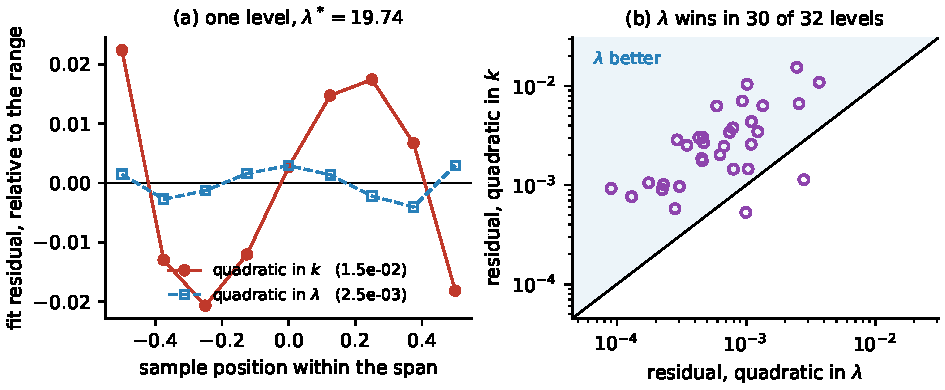
\includegraphics[width=\textwidth]{refinevar.pdf}
  \caption{\emph{(a)} Residuals of a quadratic fit to $\sig_1^2$ at one level, over the same
  nine physical points, in $k$ and in $\lam$. The fit in $k$ leaves a systematic W-shaped
  residual an order of magnitude larger. \emph{(b)} The same comparison at every isolated
  level of four rectangles.}
  \label{fig:refinevar}
\end{figure}

This deserves an honest note, because it contradicts the model. Writing the cone as
$\sig_1\approx\sqrt{\varepsilon^2+c^2(k-k^*)^2}$ makes $\sig_1^2$ exactly quadratic \emph{in
$k$}; the data say it is closer to quadratic in $\lam$. Fitting the model form directly leaves
a residual of $1.5\times10^{-2}$ against $8.7\times10^{-4}$ for a plain quadratic in $\lam$ on
the same points. So \eqref{eq:cone} is a good local model stated in a slightly wrong variable,
and the two stages of the search are entitled to disagree about which variable they want
because they are using different features of it.

\subsection{Tolerance, and the guards}

The stopping tolerance is
\begin{equation}\label{eq:xatol}
  x_{\text{atol}} \;=\; \max\bigl(\pr\cdot\abs{\lam},\ 4\,\mathrm{ulp}(\lam)\bigr).
\end{equation}
The second term is not decoration: a tolerance derived from $\lam$ alone can \emph{exceed} the
bracket it is refining --- a $2.7\times10^{-13}$ bracket handed a tolerance of
$7.9\times10^{-13}$ --- so the refiner terminates before doing anything and returns a point
that is not the minimum.

Four guards, each named with the failure it prevents.

\begin{enumerate}
\item \textbf{Refuse when the parabola never closed.} A non-positive leading coefficient means
the three points do not describe a single minimum: an empty bracket, or one holding two
well-separated eigenvalues where the fit is across a W. In the second case the lowest sampled
point can be a bracket \emph{endpoint}, far from either eigenvalue, and would be returned as a
success.
\item \textbf{But only when there was no progress.} The same condition also fires at the
\emph{end} of a good refinement, once the three points have collapsed onto the floor and the
curvature is gone. Treating that as failure discards correct answers.
\item \textbf{Track the lowest point seen independently.} The triple is re-formed by position
rather than by value, so a bad vertex can otherwise discard the sub-interval holding the
minimum.
\item \textbf{Accept against the cone outside the bracket}, where it must be rising --- not
against the bracket's own ends, which are all near the floor once the bracket is narrow.
\end{enumerate}

\subsection{The interiority trap}
\label{sec:interiority}

The last guard has a subtlety that produced the same bug twice, in two forms, and it
generalizes past this algorithm.

The naive version demands that an accepted minimum be strictly interior to its bracket. But a
bracket is guaranteed to \emph{contain} the eigenvalue, not to have the eigenvalue comfortably
inside it: the cover loop stops on purity-by-width, and a well $10^{-7}$ wide can sit inside an
$8.6\times10^{-7}$ bracket with its minimum very near an end. An interior-minimum rule discarded
8 of 26 correct brackets.

The refined version of the same error is subtler. Probe interiority by evaluating at
$x\pm h$ for a \emph{fixed} relative step $h=10^{-9}k$ and demanding both exceed $f(x)$. This
demonstrates interiority only when the located root is already nearer the true minimum than $h$
is; otherwise one step moves \emph{toward} the minimum, reads lower, and the genuine root is
refused. On an L-shape window this threw away all three eigenvalues at the default setting,
every one of which had been located to at worst $1.2\times10^{-8}$.

The right way to state the finding is as a separation rather than a threshold. The kept and
dropped populations split by a factor of eight in the ratio (location error)/$h$ --- $0.000$ to
$0.098$ against $0.782$ to $2.974$ --- but \emph{not} at $1$, because the probe compares tension
values on flanks of unequal slope. A first version of the corresponding test asserted
$\text{error}>h$ exactly and was falsified by the row at $0.78$; what survives is the mechanism
and the separation, not a constant.

\begin{remark}
The lesson generalizes, and it is the one to take away from this section. A probe whose reach
is set by the bracket width cannot know what it is stepping across. A probe whose reach is set
by a \emph{constant} cannot know that either, and additionally cannot know how accurate the
point it is stepping from is. The acceptance test that survives compares the candidate against
the two \emph{sampled} endpoints it already has, and asks nothing new of the objective.
\end{remark}

\section{Cost, and the shape of the claim}
\label{sec:claim}

\subsection{Cost}

Including the refinement each bracket hands on, at $\pr=10^{-8}$ on real pencils:
\begin{center}
\begin{tabular}{lrr}
\toprule
window & eigenvalues & evaluations per eigenvalue\\
\midrule
a resolvable pair, $\lam\in[10,88]$ & 4 & 27\\
a multiplicity-3 cluster at $50\pi^2\pm3\%$ & 3 & 27\\
a wide window, $\lam\in[10,520]$ & 35 & 26\\
\bottomrule
\end{tabular}
\end{center}
Roughly 26 evaluations per eigenvalue, near-flat in window size and in $\pr$ from $10^{-3}$
to $10^{-14}$. For comparison, a uniform grid dense enough to detect everything costs about 43
per eigenvalue \emph{and fails purity}, and grid-then-bisect costs 74--95 \emph{and loses a
third of the eigenvalues}.

\subsection{The claim, stated conditionally}

By Proposition~\ref{prop:nolipschitz} the completeness claim is not a theorem, and it must be
reported as what it is:

\begin{quote}
No $x$ in $[a,b]$ with $\sig_1(x)\le\tau$ exists outside the returned set, \emph{given} the
Lipschitz constant $L$.
\end{quote}

Every run therefore reports $L$, the largest observed secant, the ratio between them, the
number of times $L$ grew after being relied upon, and the evaluation count. A large margin
means the scan was conservative; a small one means the constant was being pushed and the run
deserves a rerun at a larger safety factor. This matters because the failure mode is silent: a
dip that is never sampled is invisible to any finite-evaluation method, and the exclusion
search in particular returns nothing after its seed, with no error at all.

\subsection{Declining is a third outcome}
\label{sec:decline}

A method may assume the objective is well behaved at the scales its precision makes relevant,
\emph{detect that it is not}, and stop. Two triggers: the seed's slope estimate never settles
(\S\ref{sec:bootstrap}), or a long run of samples buys no reduction in the unresolved regions.

Declining is neither a pass nor a failure, and it is only honest if reported. A method that
declines whenever it is about to be wrong has a perfect record over what it accepted and has
demonstrated nothing, so the decline rate is quoted beside the pass rate over the same case set,
always.

There is a related and easily conflated case which is \emph{not} a decline: being asked for
more precision than the objective can deliver. If the pencil's floor is binding, the right
answer is to emit the brackets found, flag them floor-limited, and report the attained
precision beside the requested one --- not to report that nothing was found.

\subsection{The band}

The method's real limitation is best stated as a band. Write $d$ for the separation of two
eigenvalues at level $x$. Then
\[
  \frac{d}{x} < \pr \ \ \text{(merging is licensed)},
  \qquad
  \frac{d}{x} > \text{the search's resolution} \ \ \text{(must split, and can)},
\]
and in between lies $\pr < d/x < \text{resolution}$: \emph{must split, and cannot}. The
band's width is the ratio of the resolution to $\pr$, so

\begin{quote}
the harder the precision requested, the wider the band of separations that cannot be handled.
\end{quote}

This is a property of the configuration rather than a tuning failure, and it is the reason the
honesty machinery of this section is not decoration. A method whose limits widen as it is asked
to do better has to be able to say so.

\section{What changed in the port}
\label{sec:port}

The algorithm was designed and measured in a standalone repository against a single family ---
the $(1+\delta)\times1$ rectangle with a plane-wave basis --- and then ported into
\code{chladni}. This section records the differences, because the gap between what was intended
and what the implementation found is usually the most useful part.

\subsection{What did not change}

Almost all of the tuned constants, which is the more surprising result: safety factor $1.5$,
straddle $0.02$, $1.5$ samples per expected gap, a 10\% settling tolerance, a 64-point seed
without a Weyl hint, six doublings, the stall and locator caps at 200, the dip ratio $0.5$,
three confirmation evaluations, five cover/locate rounds, an isolation clearance of four
bracket widths, and a gate margin of $1.5$. The port is a set of \emph{structural} corrections,
not a retuning.

\begin{remark}
The gate margin deserves a footnote, because it invites a misreading: the originating module's
own constant reads $2.0$, but the searcher that uses it already defaulted to $1.5$. The
constant that ships is unchanged.
\end{remark}

\subsection{Genuine differences}

\begin{longtable}{P{0.17\textwidth}P{0.29\textwidth}P{0.42\textwidth}}
\toprule
& original & \code{chladni} v1, and why\\
\midrule
\endfirsthead
\toprule
& original & \code{chladni} v1, and why\\
\midrule
\endhead
architecture & an append-only \code{Evidence} store; every component a pure function of it,
returning \code{NeedSample(x)} rather than evaluating &
flat sample arrays with cover/locate/confirm in rounds, and a view object sharing the caller's
cache at the $\lam\leftrightarrow k$ seam. Offline testability traded for fitting the
project's stage seams and a single shared, counted objective.\\[2pt]
vertex & the parabolic vertex through the raw triple &
solves for the quadratic coefficients by divided differences and \emph{requires the leading
coefficient to be positive}: a non-convex fit means the triple does not describe a single
minimum.\\[2pt]
fallback when the fit fails & sample the prediction, or the triple's midpoint &
\textbf{bisect the wider side}. Using the straddle as a fallback shrinks the bracket by 2\% per
evaluation --- measured creeping $6.2\times10^{-8}\to3.4\times10^{-8}$ over twelve evaluations,
then stopping.\\[2pt]
straddle side & gaps to the nearest evidence samples & gaps to the certificate triple's own
endpoints.\\[2pt]
multiplicity reading in the gate & a parameter, defaulted to off & removed outright: a knob
whose only safe setting is ``off'' is not a knob; see \eqref{eq:ambiguous}.\\[2pt]
slope-growth cap & 4, then decline & 16. Growth is \emph{cost, not error}, because exclusions
are recomputed from the current $L$ every pass. On a multiplicity-3 cluster the seed settles at
$0.31$ against a true wall slope of $0.683$ and needs 7 growths to reach the right answer; at 4
it declined having found nothing, at 8 it passes at 80 evaluations.\\[2pt]
exhaustion & abort & emit what is held, flag it floor-limited, and report the attained
precision beside the requested one.\\[2pt]
budget & an in-flight cap on a counted objective & 600 evaluations \emph{per expected
eigenvalue}, never flat. A flat cap silently penalises dense windows, and once turned a
38-evaluation miss into the recorded claim that a whole family was unhandleable.\\[2pt]
diagnostics & version-tagged benchmark tables & required output: $L$, its history, growths
after use, the largest secant, attained against requested precision. The completeness claim is
conditional on $L$, so $L$ must be reported.\\[2pt]
refiner start & --- & the deepest \emph{cached} sample rather than the arithmetic midpoint. A
bracket is guaranteed to contain the eigenvalue, not to have a sampled descent inside it; this
moved a located value from $1.8\times10^{-10}$ to $7.4\times10^{-12}$.\\[2pt]
refiner interior margin & --- & removed (\S\ref{sec:interiority}). It refused genuine
off-centre minima --- a level $8.8\times10^{-8}$ from a bracket end against a demanded
$2.15\times10^{-7}$ --- and was redundant with the test that the best value beat both ends.\\
\bottomrule
\end{longtable}


\subsection{Defects the port introduced, and what caught them}

These are not differences of design; they are bugs the reimplementation created and the test
tiers found. They are listed because each was found \emph{by running, not by reading}, and
because each is a plausible thing to do again.

\begin{itemize}
\item The budget defaulted to one eigenvalue where the objective offered no Weyl count, so the
locator exhausted it and returned partial results \emph{silently}.
\item Regions were retired by overlap, so bracketing one member of a pair retired the whole
region and lost the other --- coverage $0.75$ on every pair, which is
\S\ref{sec:gate}'s own failure mode arriving through the bookkeeping.
\item The fast and slow paths were collapsed. The straddle places its sample at a predicted
vertex, so on a region holding two wells it piles samples onto one and never lands between
them: coverage $1.00$ with purity failing at every precision. A region the gate has not
certified must go back to the exclusion ladder.
\item ``Silence is not permission'' applies on the way \emph{out} of the locator too: with the
post-check unable to certify, keeping the narrowed bracket discarded whatever else the region
held.
\item A region lying entirely \emph{inside} a well reads as flat --- every sample on the floor,
internal ratio $\approx1$ --- and was dropped by the confirmation step. Flatness at the floor is
the opposite of flatness on the plateau, which is why the level test is a fraction of the
measured plateau (Remark~\ref{rem:nothreshold}).
\item The loop budget counted cache \emph{misses}, so a refiner re-reading known points spun
forever at zero cost.
\end{itemize}

\subsection{Three stopping rules kept as comments}

The implementation records three rules that were tried and removed, each with the number that
removed it: a positive threshold on the envelope (broke 66 of 66 cases,
Remark~\ref{rem:zerothreshold}); a flat-bottom stop derived from $4\sig_{\min}/c$, whose
estimate is an \emph{upper} bound on the floor and so stopped narrowing far too early; and a
prominence stop on the certificate triple, which is sound in principle and unsafe early for the
same reason the further-flank normalization exists. Recording a rejected idea beside the code,
with its measurement, is what makes the design legible; it is also why the list in
\S\ref{sec:port} could be written at all.

\section{What is derived and what is measured}

A reader who takes one thing from this note should take the difference between these two
columns, because the algorithm's constants were all measured on \emph{one} family and several
still carry recalibration notes.

\begin{center}
\begin{tabular}{P{0.46\textwidth}P{0.46\textwidth}}
\toprule
\textbf{Follows from the model} & \textbf{Measured, and may not transfer}\\
\midrule
$p=1/2$ is the unique power making the wall slope level-independent, \eqref{eq:pderivation} &
that the spread in $k$ is as small as 5--6\%, and the value $C\approx0.27$\\
the envelope and its minimizer, Lemma~\ref{lem:envelope} & that $L$ from the largest secant is
nearly tight\\
the ladder ratio $(s+1)/(s-1)$, independent of $c$, Proposition~\ref{prop:ladder} & safety
$s=1.5$, gate margin $1.5$, straddle $0.02$\\
$\sig_1^2$ quadratic $\Rightarrow$ an exact vertex from three points & that $\lam$ beats $k$
for the fit (30 of 32 here, 17 of 17 there)\\
the precision factor $\pr_u=p\cdot\pr$, \eqref{eq:precu} & ${\sim}26$ evaluations per
eigenvalue\\
the cancellation-free $c$, \eqref{eq:clocal} & that $\sig_2/c$ under-reads where it errs\\
$\sig_2/\sig_1 = 1+d/u$, \eqref{eq:ambiguous} & the $\abs{\Om}/\abs{\partial\Om}$ constant
$\kappa\approx2.6$\\
\bottomrule
\end{tabular}
\end{center}

The originating design's own summary of its position is worth quoting, because it is the right
posture toward every number above: the largest uncertainty is not in any of the individual
measurements, but in the fact that all of them come from one rectangle. Several have since been
re-measured on the disk, the equilateral triangle and the L-shape; the ones that have not are
the ones to check first.

\section*{Sources}
\addcontentsline{toc}{section}{Sources}

The design records are \code{docs/design/CHLADNI\_V1.md} (the bracketing spec and its as-built
deltas), \code{docs/design/search.md} (the precision contract, the ground-truth definition, and
the multiplicity and collapse rules not developed here) and \code{docs/design/candidates.md}
(the stage seams and the comparison protocol). The implementation is
\code{tests/v1\_bracket.py} and \code{tests/v1\_refine.py}, which live in \code{tests/} because
a scored candidate lives there until it wins. Figures are regenerated by
\code{docs/figures/make\_bracket\_figures.py}, which drives the same code the text describes and
prints every number quoted in a caption.

Not developed here, and specified in \code{search.md}: the multiplicity stage, which reads
$\sig_{j+1}/\sig_j$ against a wide bracket at zero additional cost; the collapse-versus-merge
rule for roots reported close together; and the $\pr$-indexed ground truth $S(\pr)$ against
which all of it is scored.

\end{document}
